\begingroup
\definecolor{archBlue}{HTML}{527F99}
\definecolor{archOrange}{HTML}{B9784F}
\definecolor{archInk}{HTML}{33414B}
\definecolor{archFaceOne}{HTML}{86A9BC}
\definecolor{archFaceTwo}{HTML}{F2D58A}
\definecolor{archFaceThree}{HTML}{F0B078}
\definecolor{archFaceFour}{HTML}{E9A4A0}
\definecolor{archLayerBlue}{HTML}{55ADF0}
\definecolor{archLayerOrange}{HTML}{F6A159}
\definecolor{archLayerGreen}{HTML}{39C59A}
\definecolor{archLayerPurple}{HTML}{A77AD0}
\begin{tikzpicture}[x=1mm,y=1mm,
  font=\sffamily\fontsize{7.5}{9}\selectfont,text=archInk,
  box/.style={draw=archInk!55,rounded corners=1mm,fill=white,
    line width=.5pt,align=center,inner sep=1mm},
  chip/.style={box,font=\sffamily\fontsize{7}{8.5}\selectfont},
  flow/.style={-{Latex[length=1.4mm]},draw=archInk!80,line width=.6pt},
  heading/.style={anchor=west,font=\sffamily\fontsize{8.5}{10}\selectfont}]
  \path[use as bounding box] (0,3) rectangle (160,-108);
  \node[heading] at (0,0) {(a) Shared graph input};
  \node[inner sep=0] at (24,-14)
    {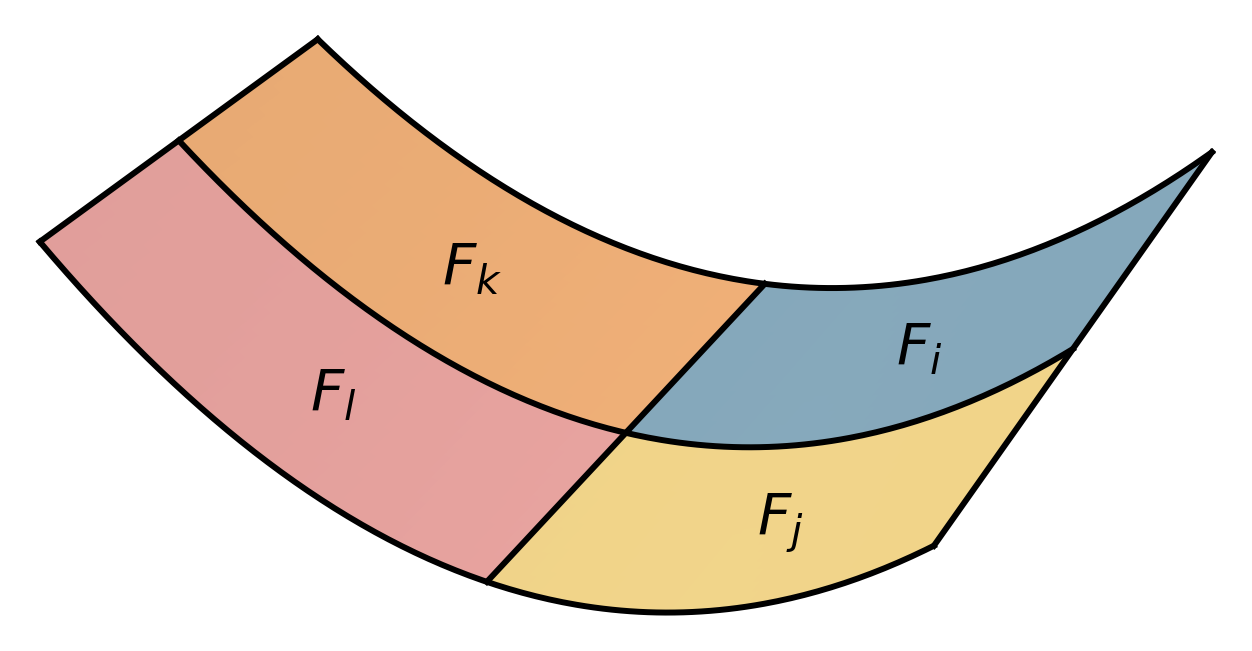
\includegraphics[width=36mm]{figures/fig5_bspline_curved_sheet.png}};
  \node[box,fill=archLayerPurple!5,text width=86mm,minimum height=20mm]
    (graphInput) at (110,-14) {};
  \draw[flow,shorten >=.4mm] (45,-14) -- (graphInput.west);
  \draw[archInk!65] (74,-8) -- (86,-8) -- (86,-20) -- (74,-20) -- cycle;
  \foreach \x/\y/\c/\f in {74/-8/archFaceThree/k,86/-8/archFaceOne/i,74/-20/archFaceFour/l,86/-20/archFaceTwo/j} {
    \node[circle,draw=archInk!60,fill=\c,minimum size=5.5mm,inner sep=0]
      at (\x,\y) {$v_{\f}$};
  }
  \node[chip,draw=archLayerBlue!65!black,fill=archLayerBlue!15,
    text width=20mm,minimum height=9mm] at (112,-14) {Node attributes\\48D};
  \node[chip,draw=archLayerGreen!65!black,fill=archLayerGreen!15,
    text width=20mm,minimum height=9mm] at (140,-14) {Edge attributes\\6D};
  \node[heading] at (0,-28) {(b) Independent GNN branches};
  \draw[draw=archInk!65,line width=.6pt] (80,-24) -- (80,-31);
  \draw[flow,draw=archBlue!85] (80,-31) -- (39,-31) -- (39,-35.7);
  \draw[flow,draw=archOrange!85] (80,-31) -- (121,-31) -- (121,-35.7);
  \fill[archInk!75] (80,-31) circle[radius=.35mm];
  \foreach \x/\col/\title/\score in {39/archBlue/Rivet branch/{p_{r,i}},121/archOrange/Small-feature branch/{p_{s,i}}} {
    \draw[draw=\col!65,fill=\col!4,rounded corners=1.5mm]
      (\x-37,-36) rectangle (\x+37,-88);
    \node[rounded corners=.8mm,fill=\col!16,text width=61mm,minimum height=5mm,
      align=center,inner sep=.4mm,text=\col!80!black] at (\x,-40) {\title};
    \node[chip,draw=\col!65,fill=archLayerBlue!8,text width=61mm,
      minimum height=5mm] (enc) at (\x,-46) {Node + edge encoders};
    \node[box,draw=\col!65,dashed,text width=61mm,minimum height=14mm]
      (conv) at (\x,-57) {};
    \node at (\x,-52) {Four NNConv layers; hidden width 64};
    % One coloured slab represents one convolution layer.
    \foreach \offset/\layer/\layerColour in {-22/1/archLayerBlue,-10/2/archLayerOrange,2/3/archLayerGreen,14/4/archLayerPurple} {
      \begin{scope}[shift={(\x+\offset,-55.5)}]
        \path[draw=\layerColour!70!black,fill=\layerColour,line width=.4pt]
          (0,0) rectangle (6.5,-6.5);
        \path[draw=\layerColour!70!black,fill=\layerColour!50!white,line width=.4pt]
          (0,0) -- (1,.8) -- (7.5,.8) -- (6.5,0) -- cycle;
        \path[draw=\layerColour!70!black,fill=\layerColour!75!black,line width=.4pt]
          (6.5,0) -- (7.5,.8) -- (7.5,-5.7) -- (6.5,-6.5) -- cycle;
        \node[font=\sffamily\fontsize{7}{8.5}\selectfont] at (3.25,-3.25) {L\layer};
      \end{scope}
    }
    \foreach \offset in {-22,-10,2} {
      \draw[flow,-{Latex[length=.9mm]}]
        (\x+\offset+7.7,-58.75) -- (\x+\offset+11.6,-58.75);
    }
    \node[chip,draw=\col!65,fill=archLayerPurple!10,text width=61mm,
      minimum height=10mm] (pool) at (\x,-71)
      {Local 64D + global mean/max 128D\\Concatenate: 192D};
    \node[chip,draw=\col!65,fill=archLayerPurple!15,text width=17mm,
      minimum height=8mm] (adapter) at (\x-22,-82) {Adapter\\$192\!\rightarrow\!96$};
    \node[chip,draw=\col!65,fill=archLayerOrange!15,text width=15mm,
      minimum height=8mm] (head) at (\x,-82) {Head\\$96\!\rightarrow\!1$};
    \node[chip,draw=\col!75,fill=\col!19,text width=18mm,
      minimum height=8mm] (score) at (\x+23,-82) {Sigmoid\\$\score$};
    \draw[flow,-{Latex[length=.9mm]}] (enc.south) -- (conv.north);
    \draw[flow,-{Latex[length=.9mm]}] (conv.south) -- (pool.north);
    \draw[flow,-{Latex[length=.8mm]}]
      (pool.south) -- (\x,-77) -- (\x-22,-77) -- (adapter.north);
    \draw[flow,-{Latex[length=.9mm]}] (adapter.east) -- (head.west);
    \draw[flow,-{Latex[length=.9mm]}] (head.east) -- (score.west);
    \draw[flow] (score.south) -- (\x+23,-92) -- (80,-92);
  }
  \node[heading] at (0,-96) {(c) Fixed threshold decision};
  \node[box,fill=archInk!3,text width=142mm,minimum height=10mm]
    (decision) at (80,-102) {};
  \node[chip,draw=archBlue!75,fill=archBlue!18,text width=43mm,
    minimum height=8mm] at (31,-102) {$p_{r,i}\geq0.90$\\Rivet};
  \node[chip,draw=archOrange!75,fill=archOrange!18,text width=43mm,
    minimum height=8mm] at (80,-102) {Otherwise, $p_{s,i}\geq0.50$\\Small-feature};
  \node[chip,draw=archInk!55,fill=archInk!9,text width=43mm,
    minimum height=8mm] at (129,-102) {Otherwise\\Background};
  \draw[flow,-{Latex[length=1mm]}] (80,-92) -- (decision.north);
\end{tikzpicture}
\endgroup
